\section{Durchführung}
Der Versuch wird nach Abbildung \ref{fig:aufbau} aufgebaut.
\begin{figure}
    \centering
    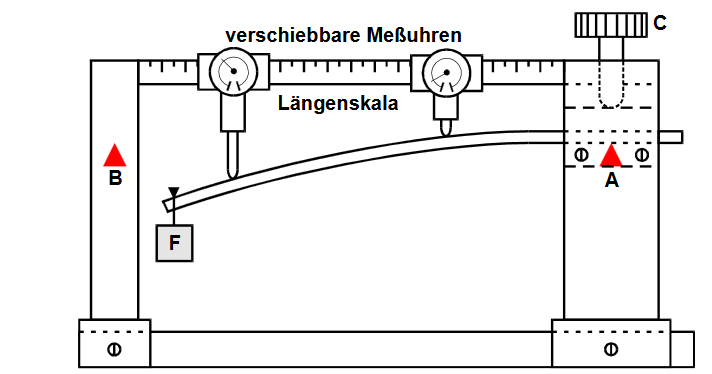
\includegraphics[width=\textwidth]{content/aufbau.png}
    \caption{Versuchsaufbau}
    \label{fig:aufbau}
\end{figure}
\noindent Der zu untersuchende Stab kann entweder in C eingespannt werden oder zwischen A und B 
aufgehängt werden.
Die Auslenkung geschieht über ein Gewicht, welches entweder am Stabende oder an der Stabmitte 
angehangen wird.
Dabei wird das Gewicht so gewählt, dass die Auslenkung sich zwischen $3$--$7\si{\milli\meter}$ 
befindet.
Diese lässt sich mit Messuhren bestimmen, welche auf der $x$-Achse beweglich sind.
Die Auslenkung wird in Abständen von $\SI{2}{\centi\meter}$ gemessen.
Es ist nicht davon auszugehen, dass die Stäbe exakt gerade sind, weshalb die Messung für 
jeden Abstand $x$ jeweils mit als auch ohne Last durchgeführt werden muss.
Die tatsächliche Auslenkung ergibt sich dann aus der Differenz der beiden Werte.
Dabei ist zu beachten, dass die Messuhren im negativen Sinn messen.
\begin{equation}
  D(x)=D_0(x) - D_M(x)
\end{equation}
Nach der Messung wird der Stab vermessen und gewogen.
